\section{Righe Spettrali}\label{sec:righe-spettrali}

\subsection{Opacità per l'atmosfera stellare}\label{sec:opacita-atmosfera}
Un parametro importante per la determinazione di un modello per l'atmosfera stellare è l'opacità, già discussa nel par.~\ref{sec:opacità}. Ripassiamo i concetti principali. I processi che determinano l'opacità di una struttura sono:
\begin{description}
    \item[BB] discusso nel par.~\ref{sec:bound-bound}. Avviene a una determinata lunghezza d'onda, secondo l'eq.~\eqref{eq:lunghezza-BB}. È responsabile delle \emph{righe di assorbimento}, poiché determinano la mancanza di flusso a una determinata lunghezza d'onda.
    \item[BF] discusso nel par.~\ref{sec:bound-free}. Contribuisce all'opacità del \emph{continuo}.
    \item[FF] discusso nel par.~\ref{sec:free-free}. Contribuisce all'opacità del \emph{continuo}.
    \item[E] discusso nel par.~\ref{sec:electron-scattering}. Contribuisce all'opacità del \emph{continuo}.
\end{description}
In particolare, nelle atmosfere le temperature sono sufficientemente basse affinché i fotoni possano essere poco energetici e possano eccitare gli elettroni degli atomi, lasciandoli in stati legati. Dunque il fenomeno del BB, che negli interni stellari trascuravamo a causa delle elevate temperatura, sarà determinante nelle atmosfere. La velocità di variazione dell'opacità con la lunghezza d'onda determina come l'opacità stessa si manifesta, ovvero in forma di righe di assorbimento o nel continuo. Vediamo degli esempi.

\paragraph{Esempio--Serie di Balmer}
\paragraph{Esempio--Balmer Jump}

\subsection{Continuo spettrale e righe spettrali di assorbimento}

\subsection{Classificazione spettrale delle stelle}
Come visto nel par.~\ref{sec:opacita-atmosfera}, l'\emph{atmosfera} stellare è dove si formano il \emph{continuo spettrale} e le \emph{righe spettrali di assorbimento}. Le righe di assorbimento, in particolare, sono degli osservabili fondamentali perché è dalla loro intensità che possiamo misurare l'\emph{abbondanza} dei diversi elementi chimici. Si faccia attenzione al seguente fatto: la presenza o meno di una data riga spettrale \emph{non} dipende dalla presenza o meno di quel dato elemento, ma è fortemente modulata dalla \emph{temperatura}. Vediamo di chiarire il fatto.

Ovviamente, se un elemento non è presente nella struttura stellare, lo spettro non potrà mostrare le sue righe. Tuttavia, l'assenza di righe di un dato elemento \emph{non necessariamente} significa che quel dato elemento è assente: potrebbe esserci, ma la \emph{temperatura} non è tale da far manifestare le sue righe. Infatti, le righe di assorbimento sono dovute a fenomeni di eccitazioni o ionizzazioni della materia e, come noto,  il numero di stati eccitati o ionizzati dipende primariamente dalla temperatura. Se, ad esempio, la temperatura non è sufficientemente alta da far sì che tutti gli atomi di un dato elemento siano ionizzati, non potrò mai vedere la riga di assorbimento di tale elemento, anche se esso è presente.

In definitiva, è la temperatura che modula il manifestarsi delle righe spettrali, ovvero è la \emph{temperatura} che determina il \emph{tipo spettrale} delle stelle. Dunque, le stelle sono classificate in base al loro tipo spettrale, ovvero in base alla presenza e all'intensità delle varie righe spettrali, il quale, a sua volta, riflette il valore della temperatura atmosferica della stella.

\begin{figure}
    \centering
    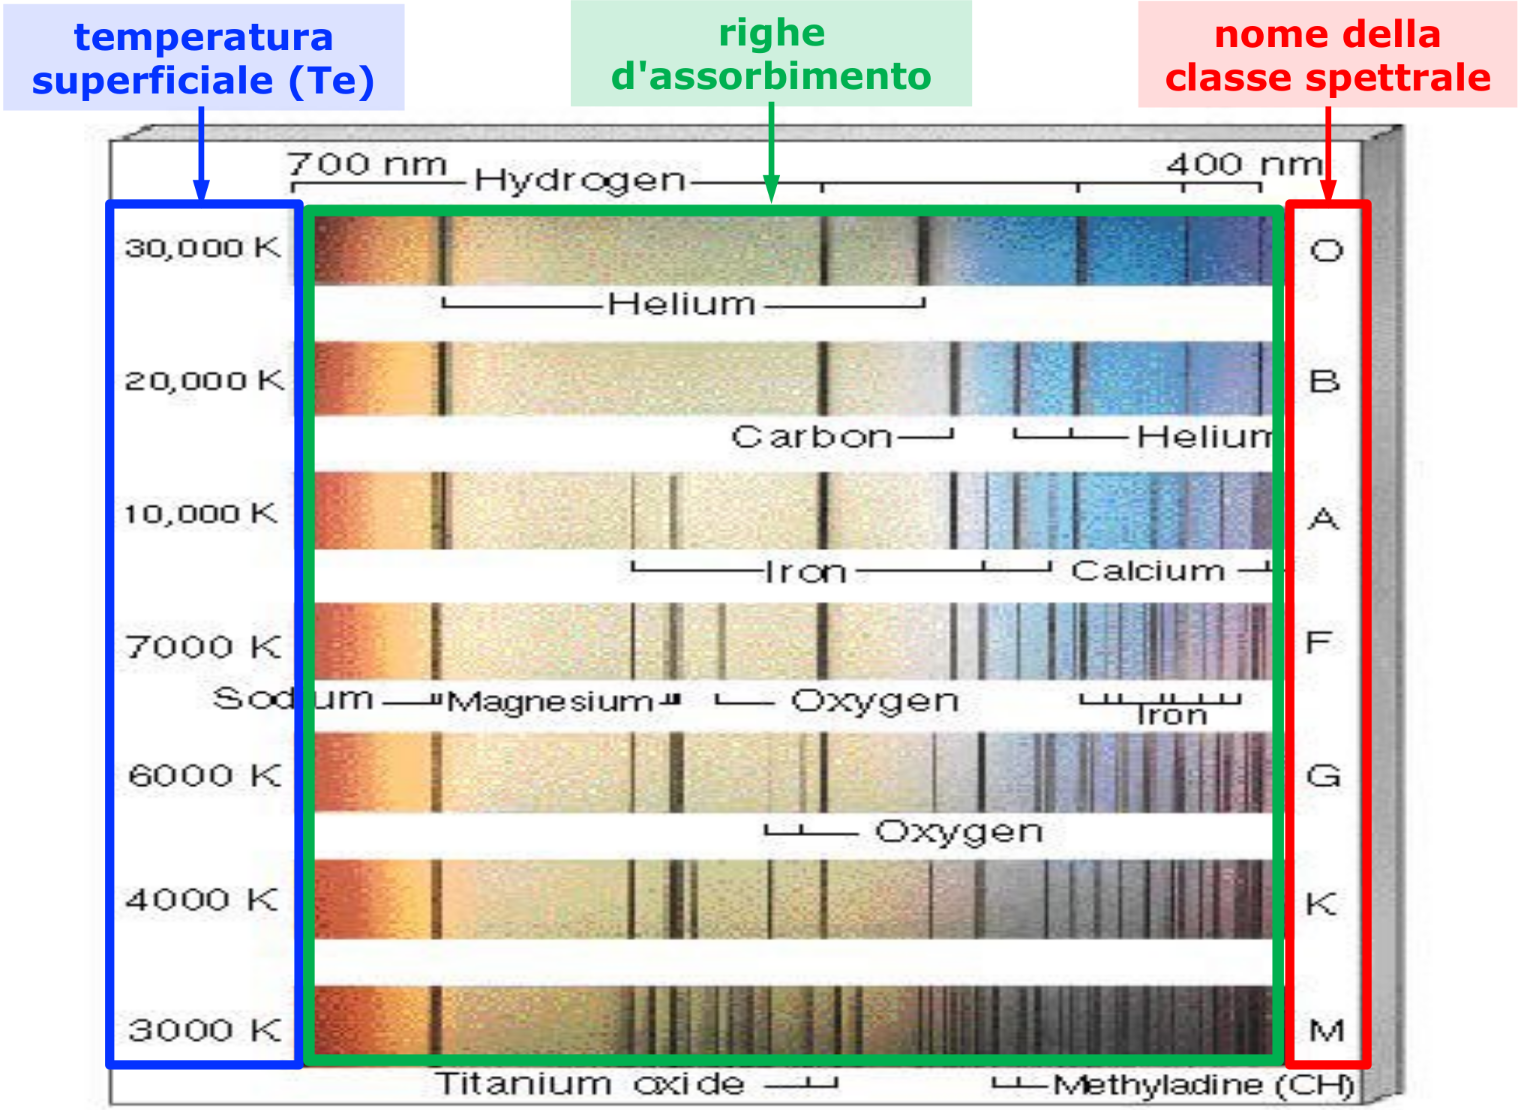
\includegraphics[width=0.6\textwidth]{immagini/classificazione-spettrale-stelle.png}
    \caption{Classi spettrali principali.}
    \label{fig:classificazione-spettrale-stelle}
\end{figure}

\begin{figure}
    \centering
    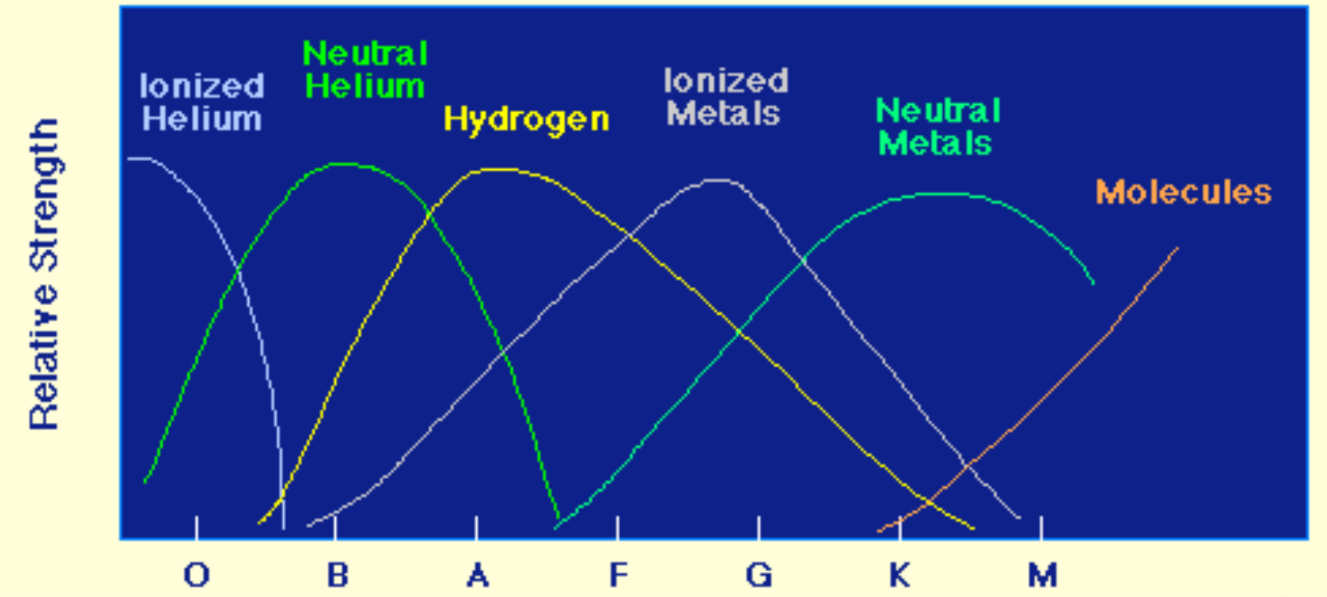
\includegraphics[width=0.6\textwidth]{immagini/classificazione-spettrale-stelle-2.png}
    \caption{Classi spettrali principali.}
    \label{fig:classificazione-spettrale-stelle-2}
    
\end{figure}

Nelle fig.~\ref{fig:classificazione-spettrale-stelle} e fig.~\ref{fig:classificazione-spettrale-stelle-2} sono rappresentate le principali \emph{classi spettrali}, elencate anche di seguito:
\begin{description}
    \item[O] $T_e > \SI{25000}{K}$
    \item[B] $ \SI{11000}{K} < T_e < \SI{25000}{K}$: ???
    \item[A] $ \SI{7500}{K} < T_e < \SI{11000}{K} $: ???
    \item[F] $ \SI{6000}{K} < T_e < \SI{7500}{K} $: ???
    \item[G] $ \SI{5000}{K} < T_e < \SI{6000}{K} $: ???
    \item[K] $ \SI{3500}{K} < T_e < \SI{3000}{K} $: ???
    \item[M] $ \SI{3500}{K} < T_e < \SI{3000}{K} $: ???
\end{description}
Si può ricordare tale lista con la seguente frase: \emph{"O,B,A, Fine Girl Kiss Me"}.

Come detto precedentemente, una data riga di assorbimento è presente o assente nello spettro a seconda del numero di atomi nei diversi stati eccitati o ionizzati di quel dato elemento. Tale numero dipende in primo luogo dalla temperatura e viene stimato attraverso:
\begin{description}
    \item[Equazione di Boltzmann]: percentuale di atomi in un dato stato di eccitazione. Risponde alla domanda: "quale frazione di atomi con elettroni legati si trova in un dato stato eccitato?"
    \item[Equazione di Saha]: percentuale di atomi in un dato stato di ionizzazione. Risponde alla domanda: "questo elemento ha ancora elettroni legati?"
\end{description}

\subsection{Equazione di Boltzmann}\label{sec:equazione-boltzmann}
Come suggerito nel precedente paragrafo, l'\emph{equazione di Boltzmann} fornisce la percenutale di atomi in un dato stato di eccitazione. In particolare, per ogni specie chimica, considera gli atomi ionizzati $j$--volte ($N_j$) e fornisce la frazioen di quelli che sono eccitati $i$--volte ($N_{ji}$):
\begin{equation}\label{eq:equazione-boltzmann}
    \dfrac{N_{ji}}{N_j} = \dfrac{g_i}{{U_j}(T)} 10^{-\theta \chi_i} 
\end{equation}
dove:
\begin{description}
    \item[$N_j$]: numero di atomi nello stato di ionizzazioni j (ovvero ionizzati $j$--volte).
    \item[$N_{ji}$]: numero di atomi nello stato di ionizzazione j, che si trovano nello stato di eccitazioni i (ovvero ionizzati $j$--volte \emph{ed} eccitati $i$--volte).
    \item[$g_i$]: peso statistico del livello energetico i.
    \item[$\theta \equiv \frac{5040}{T} \si{eV^{-1}}$], con $T$ espressa in $\si{K}$.
    \item[${U_j}(T)$]: funzione di partizione per lo stato di ionizzazione j.
    \item[$\chi_i$]: potenziale di eccitazione dal primo livello energetico disponibile al livello energetico $i$.      
\end{description}
Notiamo che l'espressione è dipendente dalla struttura dell'atomo, attraverso i termini $g_i$, ${U_j}(T)$ e $\chi_i$, e dalla temperatura. In definitiva, la percentuale è tanto maggiore quanto più alta è $T$ e quanto più basso è il potenziale di eccitazione $\chi_i$. Vediamo, ora, i vari termini con maggior dettaglio.

\paragraph{Peso statistico}
Il peso statistico $g_i$ del livello energetico $i$--esimo rappresenta il numero di livelli energetici degeneri, ovvero alla stessa energia. Per gli atomi idrogenoidi si ha:
\begin{equation*}
g_i = 2 i^2
\end{equation*}
e si ottengono i noti risultati per cui il nel livello fondamentale ($i=1$) si ha $g_1 = 2$, ovvero possono alloggiare $2$ elettroni di spin opposto, mentre nel primo livello eccitato, $i=2$, vale $g_2=8$ e possono alloggiare $2$ elettroni nell'orbitale s e $6$ elettroni nell'orbitale p, e così via.

\paragraph{Funzione di partizione}
La funzione di partizione per lo stato di ionizzazione $j$--esimo, ${U_j}(T)$, è una sommatoria dei pesi statistici ($g_i$) di tutti i livelli energetici pesati con un termine che dipende dalla temperatura, ovvero:
\begin{equation*}
    {U_j}(T) = \sum_i g_i 10^{-\theta \chi_i}
\end{equation*}

\paragraph{Potenziale di eccitazione}
nell'equazione~\eqref{eq:equazione-boltzmann}, $\chi_i$ rappresenta il potenziale di eccitazione dal primo livello energetico \emph{disponibile} al livello energetico $i$--esimo. Vediamo cosa si intende per primo livello disponibile, il quale dipenderà dal livello di ionizzazione, j. Consideriamo, ad esempio, \ce{NeI}, ovvero il neon neutro. Esso ha 10\ce{e^-} legati, in cui $2$\ce{e^-} si trovano nel livello $n=2$ e $8$\ce{e^-} si trovano nel livello $n=2$. Essendo, dunque, i primi due livelli totalmente occupati, il primo livello disponibile sarà $n=3$. Nel caso di \ce{NeII}, ovvero del neon ionizzato $1$ volta, il primo livello disponibile è $n=2$, non essendo questa volta occupato del tutto. 

Per gli atomi idrogenoidi, il potenziale di eccitazione tra due livelli energetici $a$ e $b$, con $a<b$, è:
\[
    \chi_{ab} = Z^2 \bigl( \dfrac{1}{{n_a}^2} - \dfrac{1}{{n_b}^2} \bigr) \times \SI{13.6}{eV}
\]
con $Z$ il numero atomico. Essendo il primo livello energetico disponibile il livello fondamentale, rappresentato da $a=1$, si ha:
\[
  \chi_i = Z^2 \bigl( 1-\dfrac{1}{i^2}  \bigr)  \times \SI{13.6}{eV}
\]

\subsection{Equazione di Saha}\label{sec:equazione-saha}
Per ogni specie chimica, l'\emph{equazione di Saha} fornisce la percentuale di atomi ionizzati $j+1$--volte ($N_{j+1}$) rispetto al numero di atomi ionizzati $j$--volte ($N_j$):
\begin{equation}\label{eq:equazione-saha}
    \log \dfrac{N_{j+1}}{N_j} = -0.176 - \log P_e - \theta \chi_i + 2.5 \log T + \log \dfrac{{U_{j+1}}(T)}{{U_j}(T)}
\end{equation}
dove:
\begin{description}
    \item[$N_j$, $N_{j+1}$]: numero di atomi nello stato di ionizzazione $j$ e $j+1$, ovvero contigui.
    \item[$P_e$]: pressione elettronica, ovvero esercitata dalla componente elettronica del gas. Si ricordi che siamo nelle atmosfere stellari, in cui il gas è sempre approssimabile come gas perfetto.
    \item[$\theta \equiv \frac{5040}{T} \si{eV^{-1}}$], con $T$ espressa in $\si{K}$.
    \item[$\chi_i$]: potenziale di ionizzazione dell'atomo ionizzato $j$--volte. ERRORE FORSE, NON DOVREBBE ESSERE CHI J??????
    \item[${U_j}(T)$, ${U_{j+1}}(T)$]: funzioni di partizione per gli stati di ionizzazione $j$ e $j+1$.
\end{description}
Si faccia molta attenzione a cosa si riferisce l'eq.~\eqref{eq:equazione-saha}. Essa \emph{non} permette di calcolare il numero di atomi in un certo stato di ionizzazione ( $N_j$ ) rispetto al numero totale ($N$) di atomi di quella specie, che sarebbe equivalente a $N_j / N$, tuttavia essa calcola il rapporto tra il numero di atomi in due stati di ionizzaione contigui ($j+1$ e $j$), equivalente a $N_{j+1} / N_j$. Per ottenere $N_j / N$ sono necessarie applicazioni successive dell'equazione di Saha tra due stati di ionizzazione contigui.

\subsection{Frazione di atomi attivi}\label{sec:frazione-atomi-attivi}
In pratica, mettendo insieme le due equazioni, per ogni equazione chimica:
\begin{itemize}
    \item l'equazione di Saha~\eqref{eq:equazione-saha} mi dice se, a quella data temperatura $T$ esistono atomi che non sono completamente ionizzati, cioè che hanno ancora elettroni legati
    \item se ciò è vero, l'equazione di Boltzmann~\eqref{eq:equazione-boltzmann} mi dice se, a quella data temperatura $T$ gli elettorni legati sono nello stato fondamentale o in quale livello di eccitazione
\end{itemize}
Insieme, le eq.~\eqref{eq:equazione-saha} e~\eqref{eq:equazione-boltzmann} forniscono la \emph{frazione di atomi attivi} $N_a$ (che generano le righe spettrali) rispetto al totale di atomi di quella specie. È possibile misurare $N_a$ attraverso un'analisi spettroscopica delle righe spettrali, dunque, in definitiva, usando le equazioni di Saha e Boltzmann è possibile ricavare l'\emph{abbondanza} di quel dato elemento chimico. 

\subsection{Analisi delle righe spettrali}
Come discusso nel par.~\ref{sec:opacita-atmosfera}, le linee spettrali sono originate dalle transizioni elettroni che di tipo bound--bound. Nelle righe spettrali sono contenute informazioni di cruciale importanza, tra cui le \emph{abbondanze chimiche} e la \emph{velocità radiale}.

\begin{figure}
    \centering
    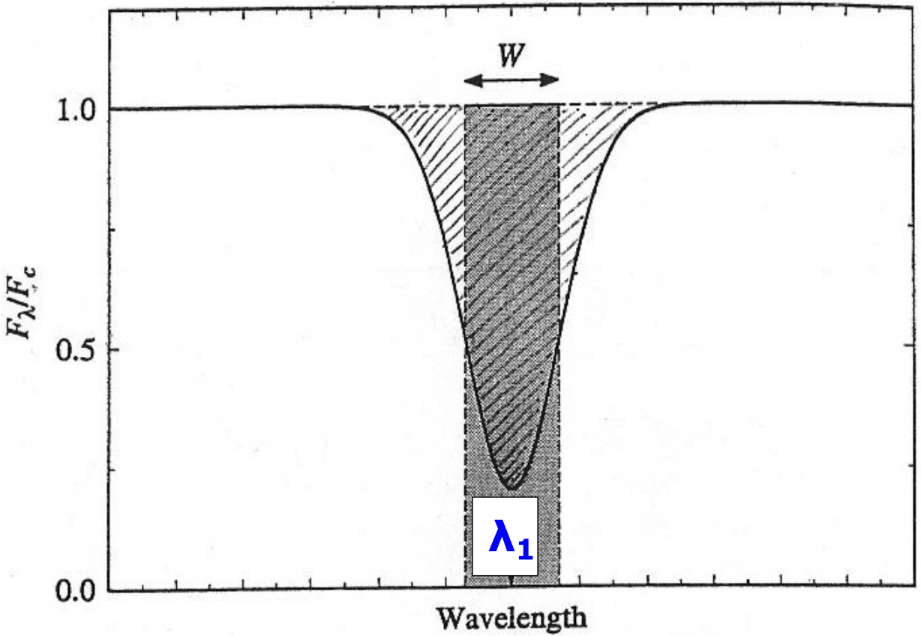
\includegraphics[width=0.5\textwidth]{immagini/righe-spettrali.png}
    \caption{Misura di una riga spettrale e analisi per la determinazione della velocità radiale e delle abbondanze chimiche. La riga spettrale di una transizione elettronica B--B è misurata a lunghezza d'onda $\lambda_1$, confrontata con la lunghezza d'onda di laboratorio di tale transizione $\lambda_0$.}
    \label{fig:righe-spettrali}
    
\end{figure}

Per capire come si procede sperimentalmente all'analisi delle righe spettrali, consideriamo una situazione tipo, illustrata in fig.~\ref{fig:righe-spettrali}. Immaginiamo di misurare una riga spettrale corrispondente a una data transizione elettronica a una lunghezza d'onda $\lambda_1$, diversa, in generale, dalla lunghezza d'onda di laboratorio di tale transizione, $\lambda_0$. A causa dell'\emph{effetto Doppler}, la differenza tra la lunghezza d'onda misurata e quella di laboratorio è una misura diretta della \emph{velocità radiale} della stella. Infatti si ha:
\begin{equation}\label{eq:effetto-doppler}
    \dfrac{\lambda_1 - \lambda_0}{\lambda_0} = \dfrac{\Delta \lambda}{\lambda_0} = \dfrac{v_r}{c}
\end{equation}

Per ciò che concerne le \emph{abbondanze chimiche}, è necessario misurare l'\emph{intensità} delle righe spettrali prodotte dagli atomi della specie studiata attraverso transizioni BB. In particolare, l'intensità, come mostrato in fig.~\ref{fig:righe-spettrali}, è rappresentata dall'area sotto la curva dello spettro continuo. È tuttavia comunemente misurata in termini di \emph{larghezza equivalente}. La larghezza equivalente $W$ è la larghezza (in Armstrong) di un rettangolo di altezza unitaria e area uguale all'intensità della riga spettrale. Si può calcolare nella seguente maniera:
\begin{equation}\label{eq:larghezza-equivalente}
    W = \int \dfrac{F_c - F_\lambda}{F_c} \ud \lambda
\end{equation} 
dove $F$ rappresenta il flusso. In particolare $W$ è correlato con il numero di atomi per $\si{cm^2}$ che generano la transizione, ovvero con $N_a$, il numero di atomi attivi. Come è possibile osservare in figura~\ref{fig:larghezza-equivalente}, la riga spettrale è tanto più profonda quanto maggiore è l'abbondanza dell'elemento considerato. Siccome la profondità della riga dipende dal numero di atomi attivi, anche $W$ dipenderà da $N_a$. In particolare è possibile osservare la loro correlazione in una \emph{curva di crescita}, mostrata in fig.~\ref{fig:curva-crescita}. Come si osserva dal grafico, l'andamento di $W$ con $N_a$ varia all'aumentare del numero di atomi attivi. Nel \emph{regime lineare} si ha $W \propto N_a$ poiché $W$ è dominata dal contributo del core della riga, evidenziato nella fig.~\ref{fig:larghezza-equivalente-regime-lineare}. Aumentando il numero di atomi attivi si entra nel \emph{regime piatto (o di saturazione)}, in cui si ha $W \propto \sqrt{\log N_a}$. In questo regime $W$ cresce molto lentamente, poiché il core della riga è saturo (la riga ha massima profondità, ovvero arriva a toccare lo zero) e il contributo delle ali è ancora trascurabile, come mostrato in fig.~\ref{fig:larghezza-equivalente-regime-piatto}. Nel \emph{regime di smorzamento} $W$ si ha $W \propto \sqrt{N_a}$ e $W$ torna ad essere più sensibile alle variazioni di $N_a$ rispetto al regime di saturazione, poiché le ali hanno un contributo dominante, come mostrato in fig.~\ref{fig:larghezza-equivalente-regime-smorzamento}.

\begin{figure}
    \centering
    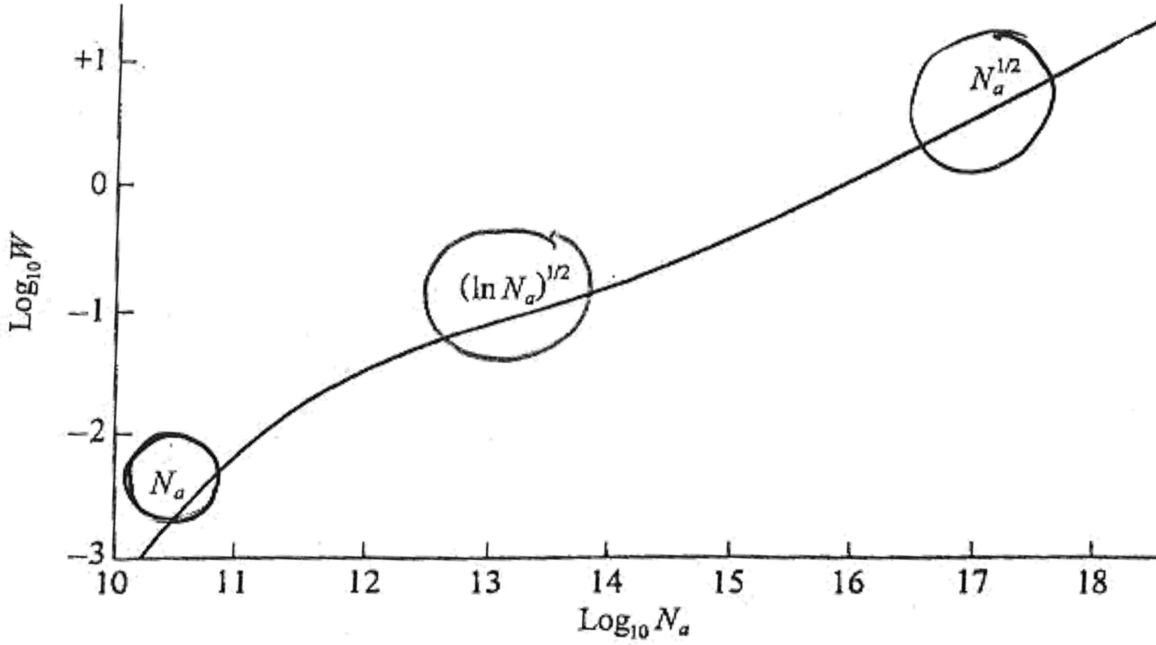
\includegraphics[width=0.5\textwidth]{immagini/curva-crescita.png}
    \caption{Curva di crescita. Descrive la dipendenza della larghezza equivalente $W$ dal numero di atomi attivi $N_a$. La curva è doppio--logaritmica. L'andamento varia con l'aumentare degli atomi attivi. In particolare, sono presenti tre regimi: il regime lineare in cui $W \propto N_a$, il regime piatto in cui $W \propto \sqrt{\log N_a}$ e il regime di smorzamento in cui $W \propto \sqrt{N_a}$.} 
    \label{fig:curva-crescita}
\end{figure}

\begin{figure}
\centering
\subfloat[][\emph{Regime lineare}\label{fig:larghezza-equivalente-regime-lineare}]
    {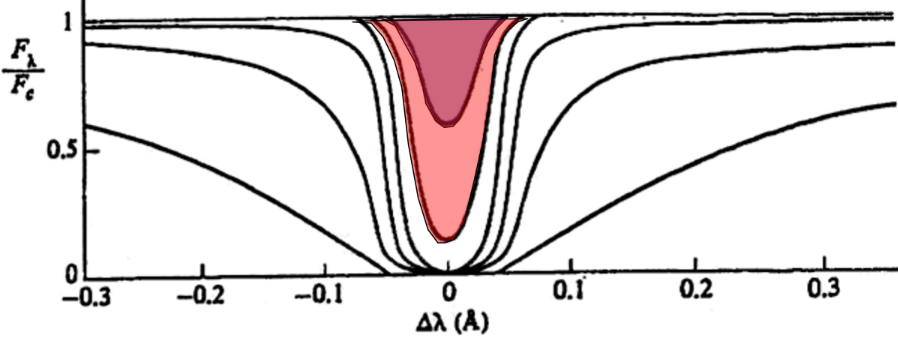
\includegraphics[width=0.45\textwidth]{immagini/larghezza-equivalente-regime-lineare.png}} \quad
\subfloat[][\emph{Regime piatto o di saturazione}\label{fig:larghezza-equivalente-regime-piatto}]
    {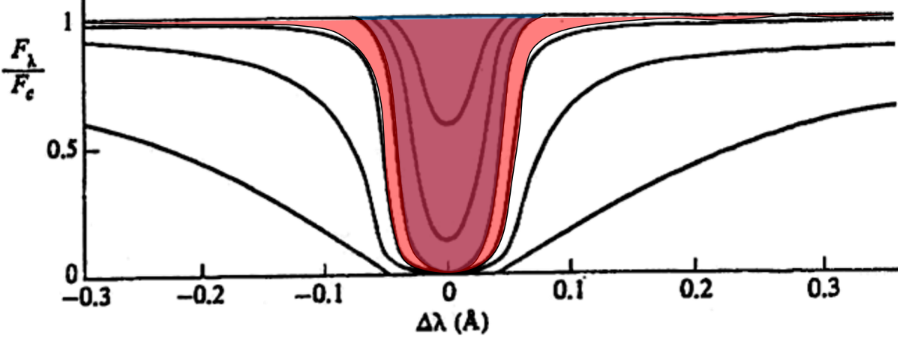
\includegraphics[width=0.45\textwidth]{immagini/larghezza-equivalente-regime-piatto.png}} \quad
\subfloat[][\emph{Regime di smorzamento}\label{fig:larghezza-equivalente-regime-smorzamento}]
    {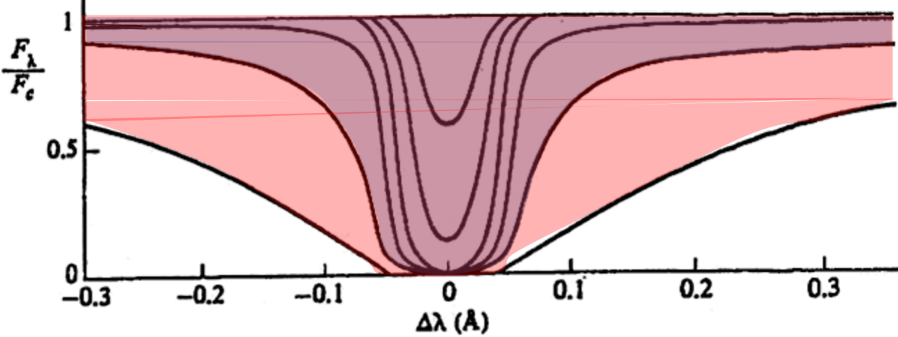
\includegraphics[width=0.45\textwidth]{immagini/larghezza-equivalente-regime-smorzamento.png}}
\caption{Correlazione tra la larghezza equivalente $W$ e il numero di atomi attivi $N_a$. La riga spettrale è tanto più profonda quanto maggiore è l’abbondanza dell’elemento considerato.}
\label{fig:larghezza-equivalente}
\end{figure}

Conoscendo la curva di crescita è possibile ricavare il numero di atomi attivi data la larghezza equivalente, che a sua volta può essere ricavata sperimentalmente dall'analisi spettroscopica del corpo in esame. Tuttavia, siamo interessati all'\emph{abbondanza} di un elemento, piuttosto che il numero dei suoi atomi attivi, $N_a$, che dipende sensibilmente dalla temperatura dell'atmosfera stellare. Ovviamente il numero totale di atomi di una data specie, $N_\textup{tot}$, \emph{non} dipende dalla temperatura. Per ottnere $N_\textup{tot}$ dalla misura di $N_a$ è necessario conoscere la percetuale di atomi di quella data specie chimica che sono nella condizione di attivare le transizioni elettroniche che generano la linea di assorbimento che si sta misurando. Abbiamo dunque bisogno di conoscere:
\begin{enumerate}
    \item la percentuale di atomi che hanno ancora elettroni legati alla struttura atomica alla data temperatura $T$, ovvero il \emph{fattore di ionizzazione}. Esso si trova con l'\emph{equazione di Boltzmann}~\eqref{eq:equazione-boltzmann} (vedi par.~\ref{sec:equazione-boltzmann}).
    \item la percentuale di atomi nei quali gli elettroni possono effettuare le transizioni osservata alla data temperatura $T$, ovvero il \emph{fattore di eccitazione}. Esso si trova con l'\emph{equazione di Saha}~\eqref{eq:equazione-saha} (vedi par.~\ref{sec:equazione-saha}).
\end{enumerate} 

A questo punto, conoscendo il numero totale di atomi di un dato elemento, $N_\textup{tot}$, è possibile trovare l'abbondanza in massa di tale elemento nell'atmosfera stellare:
\begin{equation}\label{eq:abbondanza-in-massa}
    A_\textup{el} = N_\textup{tot} m_\textup{el}
\end{equation}
dove $N_\textup{tot}$ è il numero di atomi per \si{cm} quadro, ovvero è espresso in \si{cm^{-2}}, $m_\textup{el}$ è la massa dell'elemento, espressa in \si{g} e $A_\textup{el}$ è misurato in \si{g.cm^{-2}}. Tuttavia, si preferisce riferirsi alle \emph{square bracket abundances}.

\subsection{square bracket abundances}
Le abbondanze in massa, espresse dall'eq.~\eqref{eq:abbondanza-in-massa}, sono tipicamente normalizzate all'abbondanza di idrogeno presente nella stella studiata e anche rispetto al rapporto nel Sole, espressi in scala logaritmica. Per fare un esempio chiaritivo, supponiamo di voler esprimere l'abbondanza del sodio in una stella. Con la eq.~\eqref{eq:abbondanza-in-massa} trovo $A_\textup{Na} = \SI{9.3e-5}{g.cm^{-2}}$. Essa è normalizzata rispetto all'abbondanza dell'idrogeno nella stella stessa, che suppongiamo essere $A_\textup{H} = \SI{1.1}{g.cm^{-2}}$, in scala logaritmica:
\[
\log \Bigl( \dfrac{A_\textup{Na}}{A_\textup{H}} \Bigr)_* \sim -4 -0 = -4    
\]
A sua volta questa quantità è riferita alla quantità analoga del nostro Sole, che in questo caso vale:
\[
    \log \Bigl( \dfrac{A_\textup{Na}}{A_\textup{H}} \Bigr)_\odot = 6.33 - 12 = -5.67
\]
Ora, il logaritmo del rapporto tra l'abbondanza del sodio nell stella normalizzata rispetto all'idrogeno e l'abbondanza del sodio nel Sole normalizzata rispetto all'idrogeno ci dà la \emph{square bracket adundance} del sodio:
\[
\Bigl[ \dfrac{\textup{Na}}{\textup{H}} \Bigr] = \log \dfrac{\Bigl(\frac{A_\textup{Na}}{A_\textup{H}}\Bigr)_*}{\Bigl(\frac{A_\textup{Na}}{A_\textup{H}}\Bigr)_\odot} = \log \Bigl( \dfrac{A_\textup{Na}}{A_\textup{H}} \Bigr)_* - \log \Bigl( \dfrac{A_\textup{Na}}{A_\textup{H}} \Bigr)_\odot = -4 -(-5.67) = +1.67
\]
ovvero, nella stella osservata il sodio è $10^{1.67} \sim 50$ volte \emph{più abbondante} che nel Sole. In generale si ha la seguente formula:
\begin{equation}\label{eq:square-bracket-abundances}
    \Bigl[ \dfrac{\textup{el}}{\textup{H}} \Bigr] = \log \Bigl( \dfrac{A_\textup{el}}{A_\textup{H}} \Bigr)_* - \log \Bigl( \dfrac{A_\textup{el}}{A_\textup{H}} \Bigr)_\odot
\end{equation}
Secondo l'eq.~\eqref{eq:square-bracket-abundances}, $[\frac{el}{H}] = 0$ significa che l'abbondanza in massa dell'elemento \emph{el} è la stessa del Sole, $[\frac{el}{H}] = -0.5$ significa che è pari a $1/3$ di quella del Sole e $[\frac{el}{H}] = -2$ significa che è $1/100$ di quella del Sole.